\documentclass{beamer}
\usepackage[latin1]{inputenc}
\usepackage{amssymb}
\usetheme{Warsaw}
\title[The Dependence of Planning Horizon on Model Accuracy]{The Dependence of Effective Planning Horizon on Model Accuracy}
\author[]{David Abel  \and Enrique Areyan \\ Kavosh Asadi  \and David Hershkowitz}
\date{December 15, 2015}
\begin{document}

\begin{frame}
\titlepage
\end{frame}


\begin{frame}{Outline}
\begin{enumerate}
	\item What is the point?
	\item Background
	\item UCT Story
	\item UCT Results
	\item RandomMDP Story
	\item RandomMDP Results

\end{enumerate}
\end{frame}

\begin{frame}{What is the point?}
\end{frame}


\begin{frame}{Background}

\end{frame}


\begin{frame}{UCT Story}
\end{frame}

\begin{frame}{UCT Results}
\end{frame}

\begin{frame}{RandomMDP Story}
The evaluation is performed on a MDP designed by the authors, called RandomMDP, specified as:
\begin{enumerate}
\item 10 states, 2 actions
\item choose next state uniformly random from 5 possible states
\item rewards $~$ uniform(0,1), sample rewards have additive Gaussian noise
\end{enumerate}
Evaluation approach:


\end{frame}

\begin{frame}{RandomMDP Results}

\begin{tabular}{cc}
our results & their results \\
	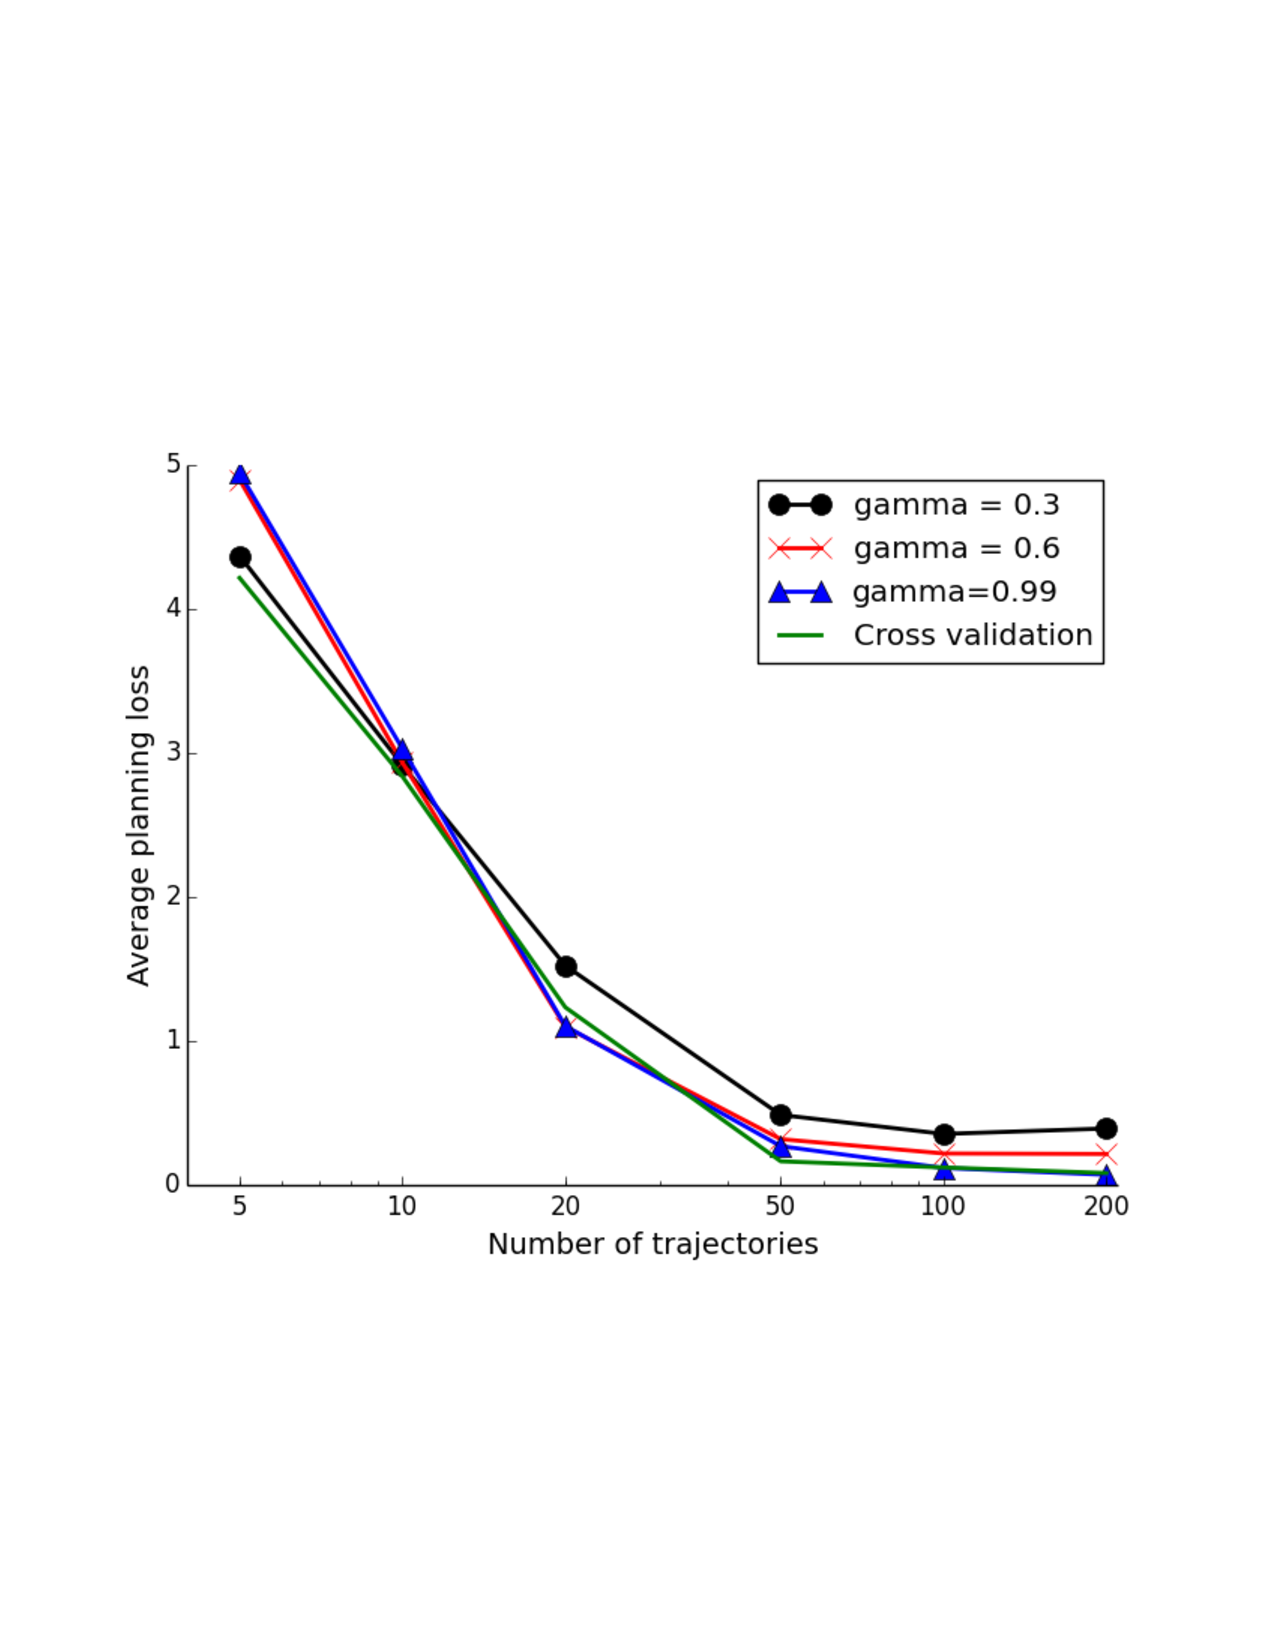
\includegraphics[page=1,height=.55\textheight,width=.5\textwidth]{../results/figure_2.pdf} &
	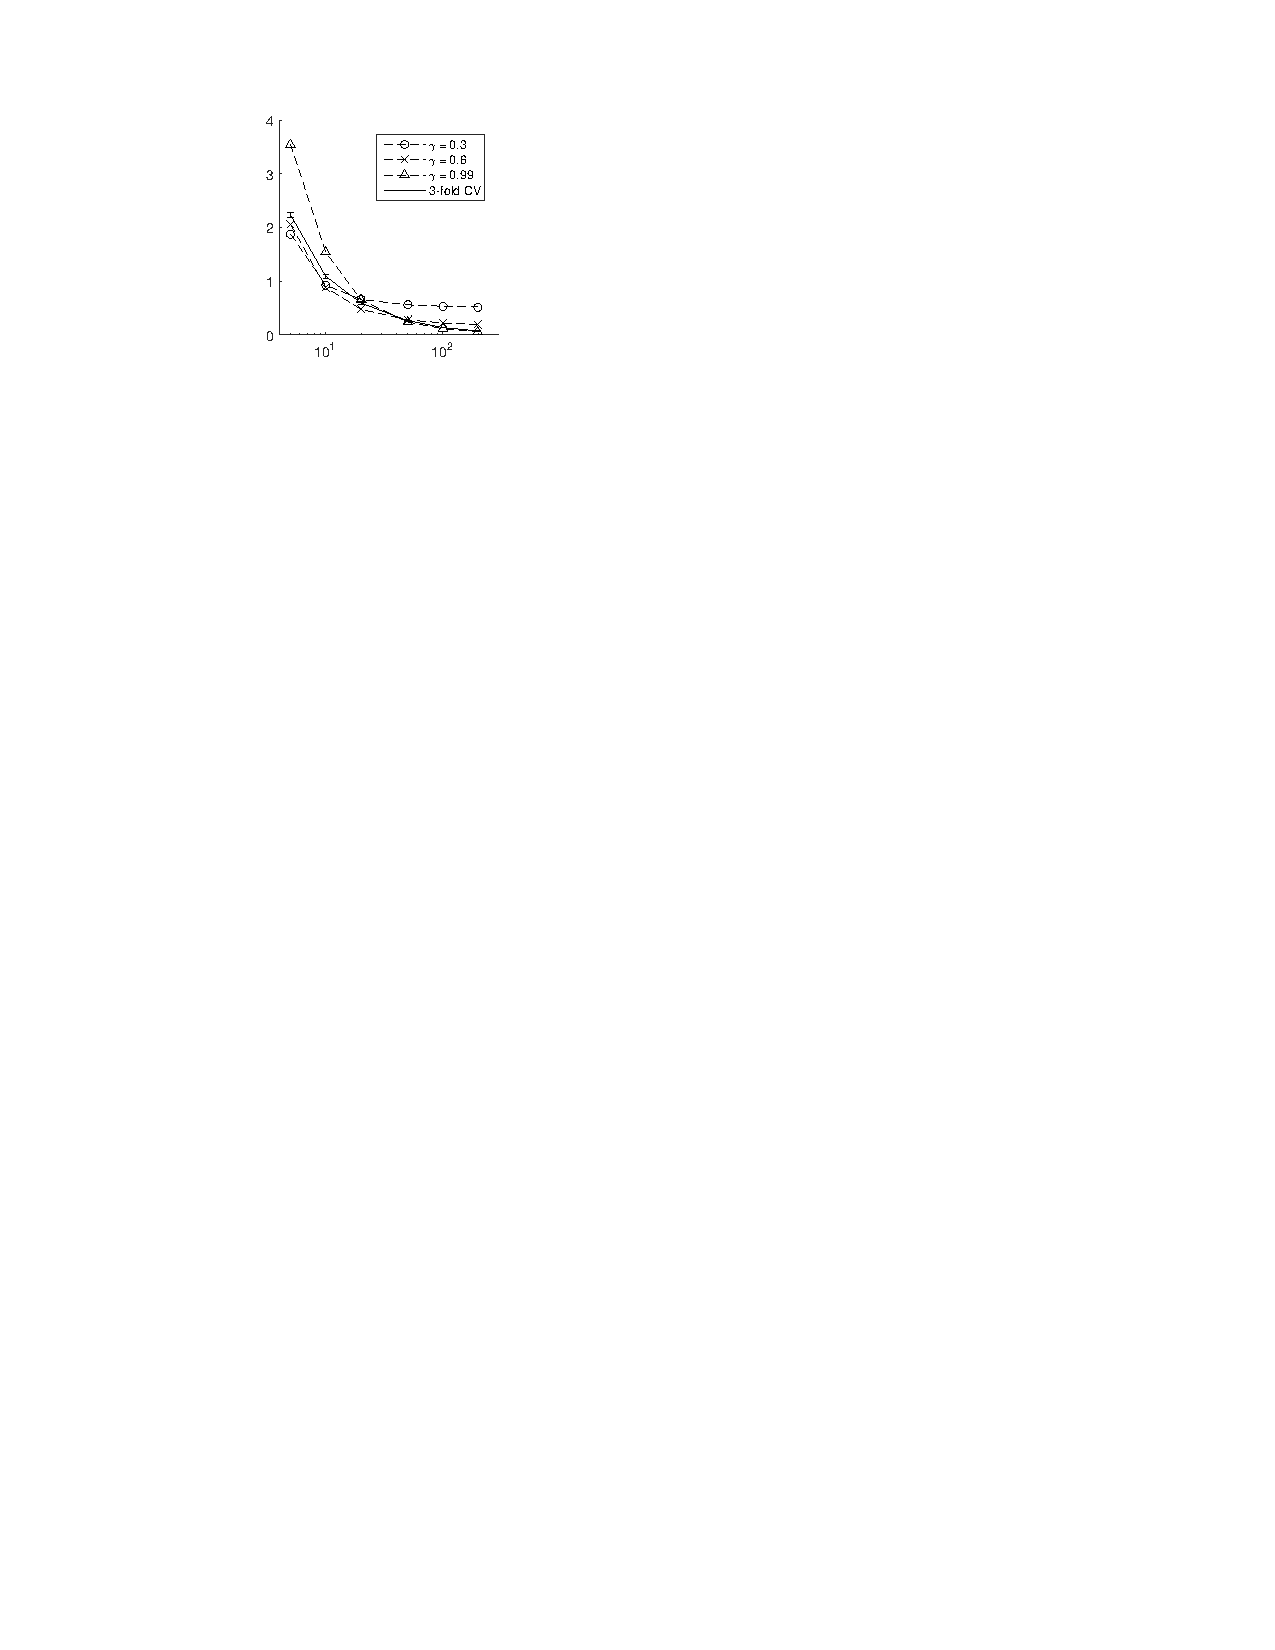
\includegraphics[page=1,width=.41\textwidth]{../results/originalCV.pdf}
\end{tabular}


\end{frame}


\end{document}
